%!TEX TS-program = xelatex
\documentclass[]{shiltemann-cv}
%\addbibresource{publications.bib}
\usepackage{fontspec}
\usepackage{verbatim}
\usepackage[dvipsnames]{xcolor}
\defaultfontfeatures{Path = /usr/share/texlive/texmf-dist/fonts/opentype/public/fontawesome/}
\usepackage{fontawesome}


\begin{document}
\header{Saskia}{Hiltemann}
    {Post-Doctoral Researcher, Bioinformatics \& Education}

% In the aside, each new line forces a line break
\begin{aside}
  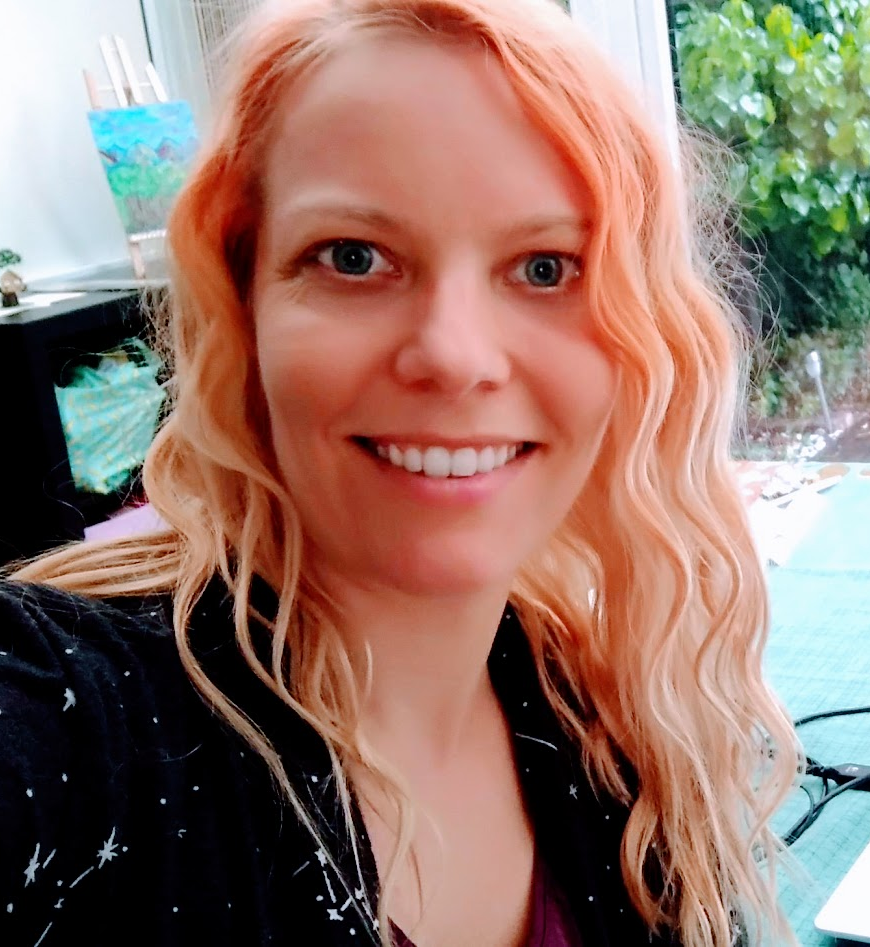
\includegraphics[width=75pt]{photo-saskia.png}
  \section{About}
    Saskia Hiltemann, Ph.D.
    ~
    Thérèse Schwartzestraat 24
    2597 XJ, Den Haag
    The Netherlands
    ~
    +31 6 33 951 365 \faPhone
    ~
    saskiahilltemann @gmail.com \faEnvelope
    @shiltemann \faGithub \ \faTwitter \ \faLinkedin
    \ \\
    ORCiD:
    0000-0003-3803-468X \faOrcid
\end{aside}

\textcolor{lightgray}{To:} \\
\color{black}
Herr Dr. Dirk Suchodoletz \\
Universität Freiburg \\
Rechenzentrum \\
Hermann-Herder-Str. 10 \\
79104 Freiburg \\


Dear Dr. Suchodoletz,

My name is Saskia, and I was happy to learn about the open position as a Coordinator for the Research Data Management Group (00003738), and would be very interested in joining the team and be a part of furthering its goals of supporting Open Science within the University of Freiburg and beyond.

In my previous positions as a Postdoctoral bioinformatician at the Erasmus Medical Center and University of Freiburg, I have gained extensive experience in research data management, across a range of scientific fields (biomedicine, plant research, metagenomics). In particular I have:

\begin{itemize}
\item Worked closely with researchers and domain experts to build FAIR and open data analysis practices, tools, and workflows, as well as data management solutions.
\item Collaborated extensively with the European Galaxy team as well as the broader Galaxy community, ELIXIR Europe, and other international partners on the development of FAIR data analysis tools, workflows, trainings and strategies.
\item Founded and coordinated the Galaxy Training Network (GTN) to not only educate researchers in the use of data analysis and -management tools, but also facilitate the \emph{FAIRifaction} of collaborative training materials from a global community of researchers and educators.
\item Organized frequent training events to improve data analysis and data management skills within the scientific research community.
\item Engaged in data stewardship tasks, most recently through the creation of DataPLANT ARCs for all projects in the MAdLand Consortium.
\end{itemize}

In addition to my extensive experience, I am also a passionate and vocal proponent of Open Science, and am confident that I could apply this experience and passion within the Research Data Management group at the University of Freiburg.

Please also find my CV included, detailing my qualifications for the position. Please do not hesitate to contact me if you have any questions, and I look forward to discussing my application with
you personally. Thank you for your time and consideration.

Best regards,

Saskia Hiltemann


\end{document}
